\section{Introduction}
\label{sec:intro}

GPU kernels are one of the main levers on the efficiency of large language model training and
serving \cite{miao2025servingsurvey}. Attention is the clearest case: each GPU generation has
required a new implementation to reach the hardware's potential, from FlashAttention on Ampere
\cite{dao2022flashattention,dao2024flashattention2} to FlashAttention-3 on Hopper
\cite{shah2024flashattention3} and FlashAttention-4 on Blackwell \cite{zadouri2026flashattention4},
each rewrite reporting a 1.5--2$\times$ speedup over its predecessor
\cite{dao2024flashattention2,shah2024flashattention3}, and serving systems ship specialized
attention engines of their own \cite{kwon2023vllm,ye2025flashinfer,miao2024specinfer}. Such kernels
are \emph{deep} targets: their performance hinges on whole-pipeline choreography (warp-specialized
producers and consumers, asynchronous tensor-core MMAs, copies ordered by barrier phases, register
budgets, persistent schedulers, the host dispatch path) rather than on local edits, their
correctness hinges on hardware invariants that documentation states only in passing, and they must
win across a production feature surface of paged caches, grouped heads, masks, ragged batches, split
decode, and low precision rather than on one shape. Domain-specific languages
\cite{tillet2019triton,spector2025thunderkittens} and template libraries \cite{nvidia2023cutlass}
lower the barrier, but state-of-the-art kernels still take expert teams months per architecture
\cite{shah2024flashattention3,zadouri2026flashattention4}, and NVIDIA's own production kernels sit
well below the hardware's speed of light on many shapes \cite{lin2026solexecbench}.

Kernel generation has therefore become an active application of LLM coding agents, with benchmarks
\cite{ouyang2025kernelbench,xing2026flashinferbench,lin2026solexecbench,oliaro2026fastkernels},
models trained with reinforcement learning to emit kernels
\cite{baronio2025kevin,li2025cudal1,cudaagent2026,drkernel2026}, agentic pipelines
\cite{hong2025autocomp,wei2025astra,kernelskill2026}, evolutionary search with an LLM as the mutation
operator \cite{novikov2025alphaevolve,lange2025shinkaevolve,chen2026avo}, and deployments across
whole production backends \cite{liao2025kernelevolve,cursor2026multiagent}. These agents sit at the
two ends of a \emph{structure--freedom} tradeoff. \emph{Scripted} agents fix in advance what the
model does at each step: a generate--test--refine loop with a learned policy
\cite{baronio2025kevin,li2025cudal1,drkernel2026}, a menu of optimizations \cite{hong2025autocomp},
a team with fixed roles \cite{wei2025astra,kernelskill2026}, or a harness in which humans gate every
promotion \cite{shui2026harness}. The script makes them sample-efficient but encodes \emph{what to
try}: Autocomp's performance collapses without its optimization menu \cite{hong2025autocomp}, and
fixed-loop RL that is competitive on single operators fails on fused models
\cite{drkernel2026,zhu2026qimengkernel,cudaagent2026}. \emph{Open-ended} agents let an LLM mutate a
population of programs
\cite{romeraparedes2024funsearch,novikov2025alphaevolve,lange2025shinkaevolve,guo2025evoengineer,wiedemann2026kernelfoundry},
and AVO makes a self-directed coding agent the variation operator itself \cite{chen2026avo}. The
freedom buys results, up to 10.5\% over FA4 for AVO \cite{chen2026avo} and a 32\% speedup of a
FlashAttention kernel for AlphaEvolve \cite{novikov2025alphaevolve}, and is paid for in trials: AVO's
agent explored more than 500 directions over seven days to commit 40 versions and needed a
supervisor to break cycles of failing edits \cite{chen2026avo}, about 30\% of the lines such agents
add are byte-identical to lines they deleted earlier \cite{pelleriti2026evotrace}, and 30--55\% of
LLM-evolved CUDA candidates are incorrect \cite{guo2025evoengineer,cuco2026}.

We argue that what both ends lack is \emph{direction}: a hypothesis about where the remaining gap
is. A script hard-codes direction and cannot supply it where the script is wrong; open-ended search
samples for it, and samples poorly, because LLMs are not open-ended optimizers. They search greedily
from their priors \cite{redko2026priorknowledge}, anchor on the solution in the prompt
\cite{jones2022cognitivebiases}, stop early out of conservatism or after a run of failures
\cite{merouani2025compilot}, cycle through near-duplicate variants
\cite{li2025tritonforge,dong2025stark}, and report completion the environment contradicts
\cite{advani2026falsesuccess}. Information is not what is missing: both ends already hand the agent
profilers, documentation, and reference implementations \cite{chen2026avo,han2026kda}, and such
feedback helps only when it supplies the specific thing the model lacks, which profiler and compiler
output rarely does \cite{redko2026priorknowledge}. What moves the same models is a hypothesis posed
from outside: intrinsic self-correction fails where external feedback succeeds
\cite{huang2024cannotselfcorrect}, a human's feedback on a model's own code raised repair success by
1.57$\times$ through structural changes the model did not propose \cite{olausson2024selfrepair}, and
in the FlashInfer kernel contest, agents given expert directions beat the same agents running alone
on every kernel \cite{shui2026harness}. Our reading, and our traces, say that a question changes the
task. ``Make this faster'' is open-ended, and the model answers it greedily. ``Is the baseline
winning on kernel cycles or only on wall-clock?'' is bounded, and to answer it the model will tear
out and rewrite a part of the kernel it would never touch on its own. A well-placed question
supplies direction without narrowing what the agent may do next, which neither more structure, more
freedom, nor more tooling can.

\begin{figure}[t]
\centering
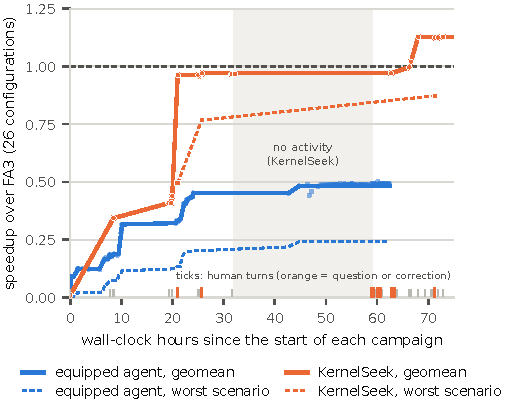
\includegraphics[width=\columnwidth]{figures/h2h.pdf}
\caption{\sys vs.\ a scripted, tool-rich autonomous agent on the same FA3 case-study task: the
same evaluator, 26 configurations, H200 node, and week. Lines are the lineage's best geomean (solid)
and worst configuration (dashed); dots are individual candidates; ticks mark human turns to \sys.
The equipped agent's model was active for the 62 hours shown; the shaded band is a period with no
\sys activity.}
\label{fig:teaser}
\end{figure}

This paper presents \sys, a question-driven agent for optimizing CUDA kernels. \sys takes an
existing kernel as its seed and makes it faster; it is not tied to an operator, and it does not need
a faster implementation to imitate. It keeps the freedom of the open-ended agents, a general-purpose
coding agent with no script and no pre-digested context, and recovers the efficiency of the scripted
ones by supplying direction at decision points: when progress stalls, when the agent claims a limit
or completion, and after suspiciously large wins. Its only purpose-built component is a minimal
harness that checks every candidate against the seed's outputs and an fp32 reference, times every
scenario against the seed, and states the goal as a stop condition that is verified rather than
requested. A good question contains no answer: it names a hypothesis the agent has not considered,
and testing it takes a measurement the agent can make with ordinary tools. Questions that recur
harden into a bank the agent applies to itself, and \sys composes with evolutionary search by
wrapping the same agent in an AVO-style lineage whose directives are questions.

We evaluate \sys on a case study chosen because a strong upstream exists to measure against:
FA3- and FA4-class attention kernels as single CUDA files with no CUTLASS, CuTe, cuBLAS, or cuDNN,
across the feature surface that vLLM exposes, with the upstream kernels as correctness oracle and
yardstick. Against an autonomous agent we built for the same task in the style of AVO and its
successors, with an orchestrated loop, pre-digested profiles, documentation retrieval, and a store
of learned lessons, \sys reached 1.13$\times$ FA3 in geometric mean over the same 26 configurations
on the same machine in the same week, where the autonomous agent plateaued at 0.50$\times$ after 133
model-driven steps (Figure~\ref{fig:teaser}). Carried through to full campaigns, \sys produced
\fathree and \fafour, correct on all 182 Hopper and all runnable Blackwell scenarios, at
1.16$\times$ FA3 and 1.46$\times$ FA4 in geomean, including 1.10$\times$ FA4 on production shapes
from SOL-ExecBench \cite{lin2026solexecbench}. Across the 16 sessions that produced them, \sys
made 11.5K tool calls per 162 human messages: asking did not mean using fewer tools, but using them
on the right thing.

\noindent This paper makes three contributions.
\begin{itemize}[nosep,leftmargin=*]
\item We identify the failure modes of autonomous agents on deep kernel targets that neither more
structure, more freedom, nor more tooling fixes, and show them co-occurring in a tool-rich agent
built to the prevailing recipe (\S\ref{sec:baseline}).
\item We present \sys, an operator-agnostic question-driven kernel agent built from a minimal
harness, a verifiable goal, and a reusable question bank, and show how it composes with
evolutionary search (\S\ref{sec:workflow}).
\item We compare \sys with the equipped agent on the same task, evaluator, hardware, and week,
analyze 162 human messages and 11.5K tool calls to show which questions redirected the agent and
why (\S\ref{sec:eval}), and release \fathree and \fafour, to our knowledge the fastest open-source
FA3- and FA4-class forward kernels on the scenarios we evaluate, with the harness, question bank,
and complete traces of both approaches (\S\ref{sec:kernels}).
\end{itemize}
